\cotefile{144}
\scanpage{168}

\[
\sigma_1,\sigma_2,\sigma,\rho_1,\rho_2
\]
\[
\left.
\begin{gathered}
\sigma_1^2=\sigma_2^2=(\sigma_1\sigma_2)^2=1\\
\sigma_1\sigma_2=\sigma^2,\quad
\sigma_1(\sigma)=\sigma_2(\sigma)=\sigma^{-1}
\end{gathered}
\right\}
\begin{array}{l}
D_\sigma\ \text{\unsure{engendré} par }\sigma_1,\sigma_2,\sigma\\[-2pt]
\shortparallel\\[-2pt]D_4
\end{array}
\]
\[
\left.
\begin{gathered}
\sigma_i(\rho_j)=\rho_{\unsure{j}}^{-1}\\
\sigma(\rho_1)=\rho_2
\end{gathered}\right|
\Rightarrow \sigma(\rho_2)=\rho_1
\]
\[
\deleted{\unsure{\sigma}}\qquad
D_\sigma*_{D_{\sigma_1}}D_{\rho_1}
\quad(\text{\unsure{engendré} par }\rho_1,\sigma_1)
\]

\figure{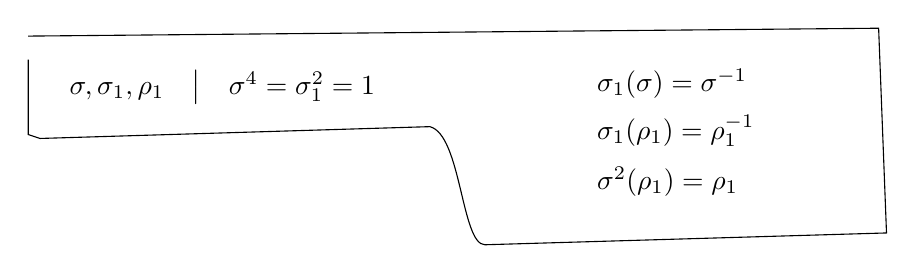
\begin{tikzpicture}[x=1cm,y=1cm]
\draw (0,2)--(10.8,2.1)--(10.9,-.5)--(5.8,-.65)
 .. controls (5.5,-.65) and (5.5,.75) .. (5.1,.85)
 --(.15,.7)--(0,.75)--(0,1.7);
\node[anchor=west] at (.4,1.35) {$\sigma,\sigma_1,\rho_1\quad\big|\quad
 \sigma^4=\sigma_1^2=1$};
\node[anchor=west] at (7.1,1.4) {$\sigma_1(\sigma)=\sigma^{-1}$};
\node[anchor=west] at (7.1,.8) {$\sigma_1(\rho_1)=\rho_1^{-1}$};
\node[anchor=west] at (7.1,.15) {$\sigma^2(\rho_1)=\rho_1$};
\end{tikzpicture}}
\[
\sigma_2=\sigma_1\underset{\text{\unsure{centre}}}{\underbrace{\sigma^2}}\ 
\unsure{\text{et}}\ \text{\unsure{commute à}}\ \sigma_1
\qquad \sigma_1\sigma_2=
\]
\[
\sigma_2(\unsure{\rho_1})=
\]

\figure{\begin{tikzpicture}[x=1cm,y=1cm]
\draw (-3,1.35)--(7.8,1.65);
\node at (-1.3,.15) {$\sigma^2-$};
\draw (1,0) ellipse (1.4 and 1.25);
\draw[->] (1,1.2)--(1,-1.15);
\draw (1.04,1.08)--(.96,-.65);
\draw[->] (2.3,0)--(-.3,.04);
\draw (1.9,-.08)--(.15,.02);
\draw[->] (2.28,-.6) .. controls (2.25,-.95) and (2,-1.13) .. (1.9,-1.15);
\end{tikzpicture}}
\[
\left\{\begin{aligned}
\sigma_1e_1&=e_1\\
\unsure{e_1|\sigma_1}e_2&=-e_2
\end{aligned}\right.
\qquad
\left\{\begin{aligned}
\sigma_2e_1&=-e_1\\
\sigma_2e_2&=e_2
\end{aligned}\right.
\qquad
\left\{\begin{aligned}
\sigma e_1&=e_2\\
\unsure{\sigma}e_2&=-e_1
\end{aligned}\right.
\]

\figure{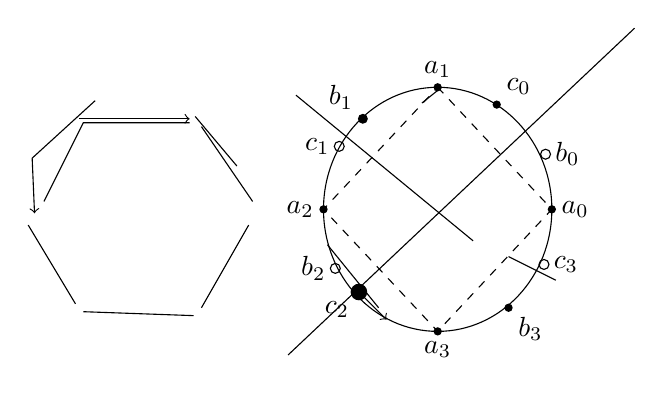
\begin{tikzpicture}[x=1cm,y=1cm]
\draw (-4,.9)--(-3.5,1.9)--(-2.15,1.9);
\draw (-2,1.85)--(-1.35,.9);
\draw (-1.4,.6)--(-2,-.45);
\draw (-2.1,-.55)--(-3.5,-.5);
\draw (-3.6,-.4)--(-4.2,.6);
\draw[->] (-3.55,1.95)--(-2.15,1.95);
\draw[->] (-3.35,2.18)--(-4.15,1.45)--(-4.12,.75);
\draw (-2.08,1.98)--(-1.55,1.35);
\draw (1,0.8) ellipse (1.45 and 1.55);
\draw[dashed] (1,2.35)--(2.45,.8)--(1,-.75)--(-.45,.8)--cycle;
\draw (-.8,2.25)--(1.45,.4);
\draw (-.9,-1.05)--(3.5,3.1);
\draw (.8,2.15)--(1.05,2.35);
\draw (1.9,.2)--(2.5,-.1);
\draw (.25,-.45)--(-.4,.35);
\fill (2.45,.8) circle (1.5pt) node[right] {$a_0$};
\fill (1,2.35) circle (1.5pt) node[above] {$a_1$};
\fill (-.45,.8) circle (1.5pt) node[left] {$a_2$};
\fill (1,-.75) circle (1.5pt) node[below] {$a_3$};
\draw (2.37,1.5) circle (1.8pt) node[right] {$b_0$};
\fill (.05,1.95) circle (1.8pt) node[above left] {$b_1$};
\draw (-.3,.05) circle (1.8pt) node[left] {$b_2$};
\fill (1.9,-.45) circle (1.5pt) node[below right] {$b_3$};
\fill (1.75,2.13) circle (1.5pt) node[above right] {$c_0$};
\draw (-.25,1.6) circle (1.8pt) node[left] {$c_1$};
\fill (0,-.25) circle (3pt) node[below left] {$c_2$};
\draw (2.35,.1) circle (1.8pt) node[right] {$c_3$};
\draw[->] (0,-.25)--(.35,-.6);
\end{tikzpicture}}
\[
\rho_1e_1=e_1\qquad
\rho_1e_2=\deleted{\unsure{e_1}}e_2-e_1
\]
\[
\unsure{\tau'_4|\sigma'_1}=
\begin{pmatrix}1&0\\0&-1\end{pmatrix}
\qquad
\underset{\substack{\shortparallel\\\tau_\infty}}
 {\unsure{\tau''_4|\sigma''_2}}=
\begin{pmatrix}-1&0\\0&1\end{pmatrix}
\qquad
\sigma=\begin{pmatrix}0&-1\\1&0\end{pmatrix}
\]
\figure{\begin{tikzpicture}\draw (0,.1)--(0,0)--(2.1,0)--(2.1,.1);\end{tikzpicture}}
\[
\unsure{\rho_0|\rho_1}=
\begin{pmatrix}1&-1\\0&1\end{pmatrix}
\deleted{\unsure{\rho_1}}
\qquad
\unsure{\sigma_1}\xi_0=\rho'\xi'_0=\xi_1
\]
\margin{168}
